\documentclass{include/thesisclass}
% Main File - Based on thesisclass.cls
% Comments are mostly in English
% ------------------------------------------------------------------------------
% Further files in folder:
%  - include/cmds.tex (for macros and additional commands)
%  - include/kitlogo.pdf (for titlepage)
%  - lit.bib (bibtex bibliography database)
%  - include/titlepage.tex (for layout of titelpage)
% ------------------------------------------------------------------------------
% Useful Supplied Packages:
% amsmath, amssymb, mathtools, bbm, upgreek, nicefrac,
% siunitx, varioref, booktabs, graphicx, tikz, multicol

%images
\usepackage{graphicx}

%for tables
\usepackage{tabularx}
\usepackage{booktabs}
\usepackage{float}
\renewcommand\thempfootnote{\arabic{mpfootnote}} %to show footnote with numbers in tables

% acronyms
\usepackage{acronym} 

%misc
\usepackage{siunitx}
\usepackage{glossaries}

%% -------------------------
%% |    Thesis Settings    |
%% -------------------------
% english or ngerman (new german für neue deutsche Rechtschreibung statt german)
\SelectLanguage{english}
% details on this thesis
\newcommand{\thesisauthor}{Olena Manzhura}
\newcommand{\thesistopic}{A Terabit sampling system with a photonics time-stretch analog-to-digital converter}
\newcommand{\thesisentopic}{Ein Terabit Abtastsystem mit Photonic-Time-Stretch Analog-Digital-Wandler}
\newcommand{\thesislongtopic}{}
\newcommand{\thesisinstitute}{Institute for Data Processing and Electronics (IPE)}
\newcommand{\thesisreviewerone}{Prof. Dr. Anke-Susanne Müller (LAS)}
\newcommand{\thesisreviewertwo}{Dr. Michele Caselle (IPE)}
\newcommand{\thesisadvisorone}{} % to use: enter names and uncomment in titlepg
\newcommand{\thesisadvisortwo}{}
\newcommand{\thesistimestart}{15.11.2020} % on titlepage
\newcommand{\thesistimeend}{14.05.2021} % on titlepage
\newcommand{\thesistimehandin}{14.05.2021} % on second page 'preamble'
\newcommand{\thesispagehead}{Master Thesis: \thesisentopic} % page heading





%% ---------------------
%% |    PDF - Setup    |
%% ---------------------
% This information will appear embed into the PDF file as meta data, but will 
% not be printed anywhere
\hypersetup
{
    pdfauthor={\thesisauthor},
    pdftitle={Masterarbeit: \thesistopic},
    pdfsubject={\thesislongtopic},
    pdfkeywords={kit,physik,bachelor,thesis,\thesisauthor}
}





%% --------------------------------------
%% |    Settings for Word Separation    |
%% --------------------------------------
% Help for separation:
% In German package the following hints are additionally available:
% "- = Additional separation
% "| = Suppress ligation and possible separation (e.g. Schaf"|fell)
% "~ = Hyphenation without separation (e.g. bergauf und "~ab)
% "= = Hyphenation with separation before and after
% "" = Separation without a hyphenation (e.g. und/""oder)

% Describe separation hints here:
\hyphenation
{
    über-nom-me-nen an-ge-ge-be-nen
    %Pro-to-koll-in-stan-zen
    %Ma-na-ge-ment  Netz-werk-ele-men-ten
    %Netz-werk Netz-werk-re-ser-vie-rung
    %Netz-werk-adap-ter Fein-ju-stier-ung
    %Da-ten-strom-spe-zi-fi-ka-tion Pa-ket-rumpf
    %Kon-troll-in-stanz
}

%% -----------------------
%% |    Main Document    |
%% -----------------------
\begin{document}
    % Titlepage and ToC
    \FrontMatter
    

    % coordinates for background border
\newcommand{\diameter}{20}
\newcommand{\xone}{-15}
\newcommand{\xtwo}{160}
\newcommand{\yone}{15}
\newcommand{\ytwo}{-253}




\begin{titlepage}
    % background border
    \begin{tikzpicture}[overlay]
    \draw[color=gray]
            (\xone mm, \yone mm)
      -- (\xtwo mm, \yone mm)
    arc (90:0:\diameter pt)
      -- (\xtwo mm + \diameter pt , \ytwo mm)
        -- (\xone mm + \diameter pt , \ytwo mm)
    arc (270:180:\diameter pt)
        -- (\xone mm, \yone mm);
    \end{tikzpicture}



    % KIT image and sign for faculty of physics
    \begin{textblock}{10}[0,0](4.5,2.5)
        \includegraphics[width=.25\textwidth]{include/kitlogo.pdf}
    \end{textblock}
    \changefont{phv}{m}{n}    % helvetica
    \begin{textblock}{10}[0,0](5.5,2.2)
        \begin{flushright}
             \large DEPARTMENT OF ELECTRICAL ENGENEERING \\ 
             AND INFORMATION TECHNOLOGY
             \\\thesisinstitute
        \end{flushright}
    \end{textblock}



    % horizontal line
    \begin{textblock}{10}[0,0](4.2,3.1)
        \begin{tikzpicture}[overlay]
        \draw[color=gray]
                (\xone mm + 5 mm, -12 mm)
          -- (\xtwo mm + \diameter pt - 5 mm, -12 mm);
        \end{tikzpicture}
    \end{textblock}



    % begin of text part
    \changefont{phv}{m}{n}    % helvetica
    \centering



    % thesis topic (en and ge)
    \vspace*{3cm}
    \Huge\thesistopic\\
    %\huge(\thesisentopic)\\



    % author name and institute
    \vspace*{2cm}
    \LARGE Master Thesis\\of\\
    \vspace*{1cm}
    \thesisauthor\\
    \vspace*{1cm}
    \LARGE at the \thesisinstitute



    % possible frontimage - thanks to JabberWok
    % for publishing the img under GNU Document License
    \vspace*{1.5cm}
    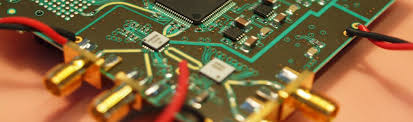
\includegraphics[scale=0.7]{./include/frontimage.png}\\



    % examiners (Referenten)
    \vspace*{1.5cm}
    \LARGE
    \begin{center}
        \begin{tabular}[ht]{l c l}
        \iflanguage{english}{Reviewer}{Referent}: 
            & \hfill & \thesisreviewerone\\
        \iflanguage{english}{Second Reviewer}{Korreferent}: 
            & \hfill & \thesisreviewertwo\\
        % uncomment if you want to provide info on your advisors
        %\iflanguage{english}{Advisor}{Betreuender Mitarbeiter}: 
        %    & \hfill & \thesisadvisorone\\
        %\iflanguage{english}{Second Advisor}{Zweiter betreuender Mitarbeiter}: 
        %    & \hfill & \thesisadvisortwo\\
        \end{tabular}
    \end{center}



    % working time
    \vspace{1cm}
    \begin{center}
        %\large{{Bearbeitungszeit}: 
        \thesistimestart \hspace*{0.25cm} -- %
                                 \hspace*{0.25cm} \thesistimeend
    \end{center}



    % lowest text blocks concerning the KIT
    \begin{textblock}{10}[0,0](2,16.8)
        \tiny{KIT – Die Forschungsuniversität in der Helmholtz-Gemeinschaft}
    \end{textblock}
    \begin{textblock}{10}[0,0](10,16.75)
        \large{\textbf{www.kit.edu}}
    \end{textblock}
\end{titlepage}

    \chapter*{Declaration}
I hereby declare that I wrote my master thesis on my own and that I have followed the regulations relating to good scientific practice of the Karlsruhe Institute of Technology (KIT) in its latest form. I did not use any unacknowledged sources or means, and I marked all references I used literally or by content.\\

\vspace{1cm}

\renewcommand{\arraystretch}{0} % for spacing in the tabular environment

\begin{flushright}
	\begin{tabular}{rr}
		Karlsruhe, \thesistimehandin, & \hspace*{5cm}\\[0mm]
		\cline{2-2}\\[2mm]    % the last line has height 2mm due
		& \thesisauthor       % to \arraystretch=0
	\end{tabular}
\end{flushright}

\vfill

\begin{flushright}
	Approved as an exam copy by \\
	\vspace{1cm}
	\begin{tabular}{rr}
		Karlsruhe, \thesistimehandin, & \hspace*{5cm}\\[0mm]
		\cline{2-2}\\[2mm]    % the last line has height 2mm due
		& \thesisreviewerone  % to \arraystretch=0
	\end{tabular}
\end{flushright}

\renewcommand{\arraystretch}{1}

\cleardoublepage

    \chapter*{Abstract}

Analysis of events occurring in the range of femtoseconds is desired in many scientific experiments.
The high temporal resolution needed for measuring such events imposes a great technological challenge for \glspl{daq} and \glspl{adc}.
In order to relax the requirements on the acquisition systems, the so-called optical time-stretch technique is used to stretch the analog input signal in time.
By using this method data converters can be operated at lower sample rate than would be required without it (several \gls{thz} to ). 
Measuring the signal with commercial \glspl{daq}, such as digital storage oscilloscopes, still poses another challenge.
Due to the limited acquisition time windows of such systems, continuous measurements at high sampling rate over a long period of time is not possible.
In applications, where measurements of the long-term evolution of the ultra-fast events with high temporal resolution is necessary, the limited memory size is a large limitation.
Therefore new concepts of \glspl{daq} based on the photonic time-stretch method need to be considered.

In this thesis, a first demonstrator of such a new photonic time-stretch based \gls{daq} system has been developed.
The system consists of a high bandwidth front-end sampling card, mounted on a back-end readout card integrating a new generation of \gls{rfsoc} for readout and processing of the acquired samples. 
%todo photonic time stretch erklären

First, the signal under study is stretched using chirped optical pulses and using the chromatic dispersion in optical fibers.
The signal is measured with a photodetector and sampled by the front-end sampling card.
The front-end sampling card integrates 16 sampling channels, each containing a \gls{tha}. 
The sampling time of these \glspl{tha} can be delayed individually.
In this way the so-called time-interleaving method can be implemented to sample the signal at a higher rate thant that normally possible due to the Nyquist theorem.
The design of the board allows it to be used with the time-stretch method as well as independently from it.
Furthermore, the setup allows for different sampling modes.
In single-channel mode one detector is connected to one sampling channel, therefore allowing to acquire data from up to 16 detectors at the same time with one sampling point per channel.
In the multi-channel mode, several channels are connected to one detector via power-splitter, therefore allowing multiple sampling points for one detector. %todo sample time

The \gls{rfsoc} on the back-end readout card integrates a processing unit and a \gls{fpga}. 
A firmware running on the \gls{fpga} is responsible for programming and controlling the components on the sampling card, as well as collecting the acquired samples and sending it to the following processing system via high-speed connections.
The processing unit, hosting e.g. an operating system or a standalone application, allows for the user to control and monitor the overall system via common periphery, e.g. Ethernet.

The name given to the system is \gls{theresa}.
The high-speed \glspl{adc}, integrated in the read-out card are capable of a sample rate of up to \SI{2.5}{\giga \sample \per \second}.
Using the time-interleaving technique for all available glspl{adc} results in an overall maximal achievable sample rate of \SI{40}{\giga \sample \per \second}.  %todo sample rate of overall system
When used in combination with the time-stretch technique and considering currently achievable time-stretch factors, a time resolution in the range of hundred of femtoseconds is possible. 
\gls{theresa} is therefore suitable to be used in beam diagnostics, e.g. at the \gls{kara}.

\chapter*{Zusammenfassung}
\chapter*{Résumé}
    
	
    \begingroup   % in order to avoid listoffigures and
    \tableofcontents                    % listoftables on new pages
    \listoffigures
    \listoftables
    \endgroup
    \cleardoublepage

	\newacronym{kit}{KIT}{Karlsruhe Institute of Technology}
\newacronym{sr}{SR}{Synchrotron Radiation}
\newacronym{linac}{LINAC}{linear accelerator}
\newacronym{rf}{RF}{Radio Frequency}
\newacronym{ipe}{IPE}{Institute for Data Processing and Electronics}
\newacronym{kara}{KARA}{Karlsruhe Research Accelerator}
\newacronym{kapture}{KAPTURE}{Karlsruhe Pulse Taking Ultra-fast Readout Electronics}
\newacronym{csr}{CSR}{Coherent Synchrotron Radiation}
\newacronym{eo}{EO}{Electro-Optic}
\newacronym{adc}{ADC}{Analog-To-Digital-Converter}
\newacronym{dac}{DAC}{Digital-To-Analog-Converter}
\newacronym{sha}{SHA}{Sample-And-Hold-Amplifier}
\newacronym{tha}{THA}{Track-And-Hold-Amplifier}
\newacronym{pll}{PLL}{Phase-Locked-Loop}
\newacronym{fmc}{FMC}{FPGA Mezzanine Card}
\newacronym{hspce}{HSPCe}{High Serial Pin Count Extension} 
\newacronym{lvcmos}{LVCMOS}{Low voltage complementary metal oxide semiconductor}
\newacronym{lvds}{LVDS}{Low Voltage Differential Signaling}
\newacronym{lvpecl}{LVPECL}{Low-voltage positive emitter-coupled logic}
\newacronym{pcie}{PCIe}{PCI Express}
\newacronym{theresa}{THERESA}{Terahertz Readout Sampling}
\newacronym{rfsoc}{RFSoC}{Radio-Frequency System-On-Chip}
\newacronym{lsb}{LSB}{Least Significant Bit}
\newacronym{dc}{DC}{Direct Current}
\newacronym{ac}{AC}{Alternating Current}
\newacronym{thz}{THz}{tera Hertz}
\newacronym{fwhm}{FWHM}{Full Width At Half Maximum}
\newacronym{fpga}{FPGA}{Field Programmable Gate Array}
\newacronym{lna}{LNA}{Low-Noise-Amplifier}
\newacronym{daq}{DAQ}{Data Acquisition System}
\newacronym{mmic}{MMIC}{Microwave Monolithic Integrated Circuit}
\newacronym{sinad}{SINAD}{Signal-to-Noise-and-Distortion Ratio}
\newacronym{snr}{SNR}{Signal-To-Noise-Ratio}
\newacronym{inl}{INL}{Integral Nonlinearity}
\newacronym{dnl}{DNL}{Differential Nonlinearity}
\newacronym{sfdr}{SFDR}{Spurious-Free Dynamic Range}
\newacronym{rms}{RMS}{Root-Mean-Square}
\newacronym{rss}{RSS}{Root-Sum-Square}
\newacronym{enob}{ENOB}{Effective-Number-Of-Bits}
\newacronym{dbfs}{dBFS}{decibels relative to full scale}
\newacronym{dbc}{dBc}{decibels relative to the carrier}
\newacronym{sjnr}{SJNR}{Signal-to-Jitter-Noise-Ratio}
\newacronym{pcb}{PCB}{Printed Circuit Board}
\newacronym{spi}{SPI}{Serial Peripheral Interface}
\newacronym{vita}{VITA}{VMEbus International Trade Association}
\newacronym{sma}{SMA}{SubMiniature version A}
\newacronym{fs}{FS}{Full-Scale}
\newacronym{ic}{IC}{Integrated Circuit}
\newacronym{emi}{EMI}{Electro-Magnetic Interference}
\newacronym{cml}{CML}{Current Mode Logic}
\newacronym{sdi}{SDI}{Serial Data Interface}
\newacronym{esr}{ESR}{Equivalent-Series-Resistance}
\newacronym{esl}{ESL}{Equivalent-Series-Inductance}
\newacronym{vcxo}{VCXO}{Voltage-Controlled Crystal Oscillator}

    % Contents
    \MainMatter
    \chapter{Introduction}
    		 \section{State of the art}
 \section{New Board}
    \chapter{Theoretical Background}
    		\section{Something about synchrotron/Terahertz radiation..?}
\section{Time-Stretch Analog-to-Digital-Converter}
	\chapter{Work}
		\begin{table}[tbh!]
	\caption{Power consumption of KAPTURE components}
	\label{tab:kapturecomp}
	\begin{minipage}{\textwidth}
	\centering
	\begin{tabular}{lccc}
		\toprule
		\textbf{Component} & \textbf{$V_{cc}$ (\SI{}{\volt})} & \textbf{$I_{max}$ (\SI{}{\ampere})} & \textbf{Power (\SI{}{\watt})}\\
			\midrule
		HMC5649 (T/H-Amplifier) 	& 2 & 0.221 & 0.442\\
								& -5 & 0.242 & 1.21\\
		LMC0480 (PLL) 			& 3.3 & 0.590\footnote{all CLKs} & 1.947\\
		HMC987LP5E (Fan-Out) 	& 3.3 & 0.234\footnote{ Outputs and RF-Buffer} & 0.772\\
		HMC856 (Delay) & -3.3 & 0.185 & -0.611 \\
		\bottomrule
		\end{tabular}
	\end{minipage}
\end{table}

    \chapter{Conclusions}
    		\subsection{Measurements with the IPE front-end card}
Card is in production. Measurements will be done, but not in the scope of the thesis.
\begin{figure}[H]
	\centering
	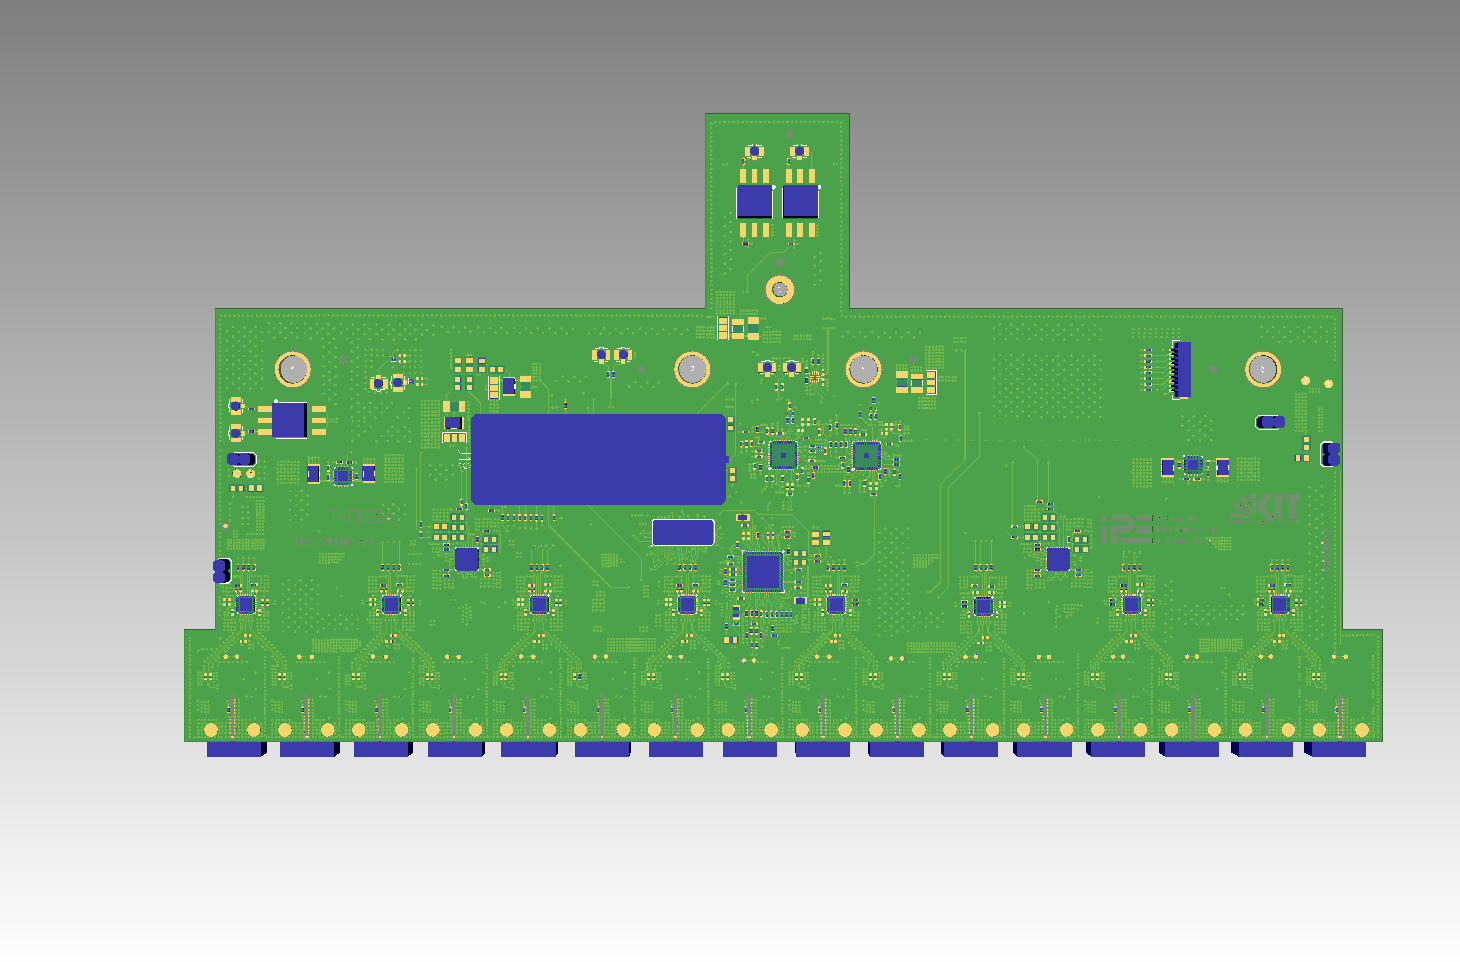
\includegraphics[width = \textwidth]{chap/05-conclusion/img/board_ugly}
	\caption{wow}
	\label{fig:board}
\end{figure}



    % appendix for more or less interesting calculations
    \Appendix
    \chapter*{\appendixname} \addcontentsline{toc}{chapter}{\appendixname}
    % to make the appendix appear in ToC without number. \appendixname = 
    % Appendix or Anhang (depending on chosen language)
    \section{First Appendix Section}
 %\cleardoublepage



    % Bibliography
    \TheBibliography

    % BIBTEX
    % use if you want citations to appear even if they are not referenced to: 
    % \nocite{*} or maybe \nocite{Kon64,And59} for specific entries
    %\nocite{*}
    \bibliographystyle{babalpha}
    \bibliography{lit.bib}

    % THEBIBLIOGRAPHY
    %\begin{thebibliography}{000}
    %    \bibitem{ident}Entry into Bibliography.
    %\end{thebibliography}
\end{document}
